\documentclass[11pt]{article}
\usepackage[a4paper,margin=1in]{geometry}
\usepackage[T1]{fontenc}
\usepackage[utf8]{inputenc}
\usepackage{lmodern}
\usepackage{microtype}
\usepackage{amsmath,amssymb}
\usepackage{booktabs}
\usepackage{enumitem}
\usepackage{graphicx}
\usepackage[hidelinks]{hyperref}
\usepackage[numbers]{natbib}
\setlength{\parskip}{0.25em}
\setlength{\parindent}{0pt}
\renewcommand{\arraystretch}{1.06}
\setlength{\textfloatsep}{8pt plus 2pt minus 2pt}
\setlength{\intextsep}{8pt plus 2pt minus 2pt}
\title{Provider-Dependent Reliability of Self-Reported Confidence under a Shared Black-Box MT Protocol}
\author{Umberto Altieri}
\date{}
\begin{document}
\maketitle
\begin{abstract}
This paper studies a trustworthy-AI reliability question for black-box language-model services: can one shared confidence threshold be reused across providers under a common protocol? We evaluate English$\rightarrow$German translation with eight models from OpenAI, Anthropic, and Google on 500 WMT17 sentences (4,000 translation--confidence pairs) at temperature 0. Quality is scored with sentence-level chrF, and low quality is operationally defined as the within-model bottom 20\% tail. Relative to that target, expected calibration error (ECE) and mismatch@0.9 differ widely despite similar mean chrF (54.0--60.1): ECE ranges from 0.076 to 0.180, and mismatch@0.9 ranges from 0.2\% to 18.2\%. The released snapshot also shows uneven parse-warning burden (443/4000 rows; 11.1\%), an implementation-level confound for cross-provider reliability comparisons. The central claim is therefore practical and scoped: under this shared protocol and operational target, self-reported confidence is provider-dependent and non-portable as a common probability scale, so a fixed threshold does not induce comparable routing/abstention operating points. Supplementary analyses indicate that provider-specific isotonic remapping can reduce ECE but does not restore portability. Limitations are explicit: operational (not semantic) target, no bundled COMET/xCOMET checkpoints, no completed semantic-audit labels, and no bundled non-baseline prompt-variant outputs.
\end{abstract}

\section{Introduction}
We study whether prompt-elicited self-reported confidence can be reused across providers as a common threshold interface for MT routing/abstention decisions. The analysis is deliberately operational: low quality is defined by reference-overlap tails, not human semantic labels. The question is practical rather than theoretical: does one threshold (e.g., 0.9) induce comparable operating points across providers under a shared protocol?

Across eight models, mean chrF is relatively clustered while confidence behavior is not. This disconnect creates portability risk: identical threshold policies can produce materially different high-confidence failure rates. We therefore treat confidence as a provider-specific decision signal unless calibrated per provider.

\section{Related work}
MT reliability work spans reference-based evaluation (e.g., BLEU/chrF), learned metrics, and QE without references. This paper does not propose a new metric or QE model; it asks whether the generating model's own confidence is stable enough for cross-provider threshold transfer \citep{blatz-etal-2004-confidence}.

In LLM settings, confidence and calibration have become central for selective prediction and abstention. Prior work shows miscalibration in modern models and motivates post-hoc correction methods; black-box settings are particularly challenging because token-level internals are unavailable \citep{ulmer-etal-2024-calibrating}.

Recent work on verbalized/self-reported confidence indicates useful signal but also sensitivity to elicitation and imperfect uncertainty expression \citep{yona-etal-2024-large}. Our contribution is a constrained MT portability test: same task, same protocol, multiple providers, and operational chrF/BLEU targets.

\section{Methods}
\textbf{Setup.} We evaluate WMT17 en$\rightarrow$de with a fixed 500-sentence sample (seed 123). Eight models (OpenAI/Anthropic/Google) each produce one translation and one scalar confidence in $[0,1]$ per sentence (4,000 outputs total). Canonical prompts and JSON schema are shared; provider adapters only handle transport.

\textbf{Operational target.} Sentence-level chrF is the primary quality signal. Low quality is the within-model bottom 20\% chrF tail. This is an operational overlap-based target, not semantic correctness calibration. A secondary robustness stage uses the strongest available alternative metric in the environment (BLEU fallback when COMET is unavailable).

\textbf{Metrics.} With 10 bins, ECE is computed against the binary non-low-quality label:
\[
\mathrm{ECE}=\sum_{b=1}^{B}\frac{|S_b|}{N}\left|\mathrm{acc}(S_b)-\mathrm{conf}(S_b)\right|.
\]
Mismatch at threshold $\tau$ is
\[
\Pr(\mathrm{low\mbox{-}quality}\wedge \mathrm{confidence}>\tau),
\]
reported mainly at $\tau=0.9$ (mismatch@0.9), a strict policy-relevant regime.

\textbf{Complexity proxy.} We include a lightweight source-side surface-complexity proxy (length/depth-like/rarity/name features) only for secondary stratification; it is not a validated semantic-difficulty measure.

Implementation details, full prompts, and script-level provenance are in the repository.

\section{Results}
Table~\ref{tab:main} shows the core result. Mean chrF is similar (54.0--60.1), but ECE (0.076--0.180) and mismatch@0.9 (0.2\%--18.2\%) vary widely. Thus a fixed threshold does not transfer cleanly across providers.

\begin{table}[t]
\centering
\small
\begin{tabular}{lcccc}
\toprule
Model & Mean chrF & ECE (within-q20) & Mismatch@0.9 & Median conf. \\
\midrule
anthropic/claude-haiku-4-5-20251001 & 57.01 & 0.094 & 13.4\% & 0.92 \\
anthropic/claude-opus-4-6 & 58.45 & 0.087 & 7.6\% & 0.93 \\
anthropic/claude-sonnet-4-5-20250929 & 56.89 & 0.095 & 12.8\% & 0.95 \\
gemini/gemini-2.5-flash & 54.01 & 0.148 & 4.2\% & 0.73 \\
gemini/gemini-2.5-pro & 60.07 & 0.180 & 18.2\% & 1.00 \\
openai/gpt-5-mini & 57.09 & 0.152 & 12.8\% & 0.93 \\
openai/gpt-5-nano & 55.31 & 0.076 & 0.2\% & 0.73 \\
openai/gpt-5.2 & 58.87 & 0.134 & 15.2\% & 0.93 \\
\bottomrule
\end{tabular}
\caption{Main summary table from regenerated code-side outputs (within-model chrF-q20 target).}
\label{tab:main}
\end{table}


Provider-specific isotonic remapping can reduce ECE for several models on held-out data, but gains are uneven and not portable; one model worsens in held-out ECE. This supports mitigation as provider-specific, not universal portability restoration.

\begin{table}[t]
\centering
\small
\begin{tabular}{lcccc}
\toprule
Model & ECE before & ECE after & Mismatch@0.9 before & Mismatch@0.9 after \\
\midrule
anthropic/claude-haiku-4-5-20251001 & 0.110 & 0.027 & 14.3\% & 0.3\% \\
anthropic/claude-opus-4-6 & 0.084 & 0.114 & 10.0\% & 2.1\% \\
anthropic/claude-sonnet-4-5-20250929 & 0.087 & 0.073 & 12.1\% & 1.0\% \\
gemini/gemini-2.5-flash & 0.152 & 0.055 & 4.9\% & 0.3\% \\
gemini/gemini-2.5-pro & 0.175 & 0.087 & 18.2\% & 0.0\% \\
openai/gpt-5-mini & 0.128 & 0.116 & 11.8\% & 0.0\% \\
openai/gpt-5-nano & 0.091 & 0.045 & 0.3\% & 0.3\% \\
openai/gpt-5.2 & 0.155 & 0.047 & 17.0\% & 0.0\% \\
\bottomrule
\end{tabular}
\caption{Held-out isotonic calibration summary from regenerated calibration artifacts.}
\label{tab:calibration}
\end{table}


Prompt-variant infrastructure and semantic-audit scaffolding are available in the repository, but non-baseline prompt outputs and completed semantic labels are not bundled in this release.

\begin{figure}[t]
\centering
\IfFileExists{figures/fig2_reliability_diagram_overlay.pdf}{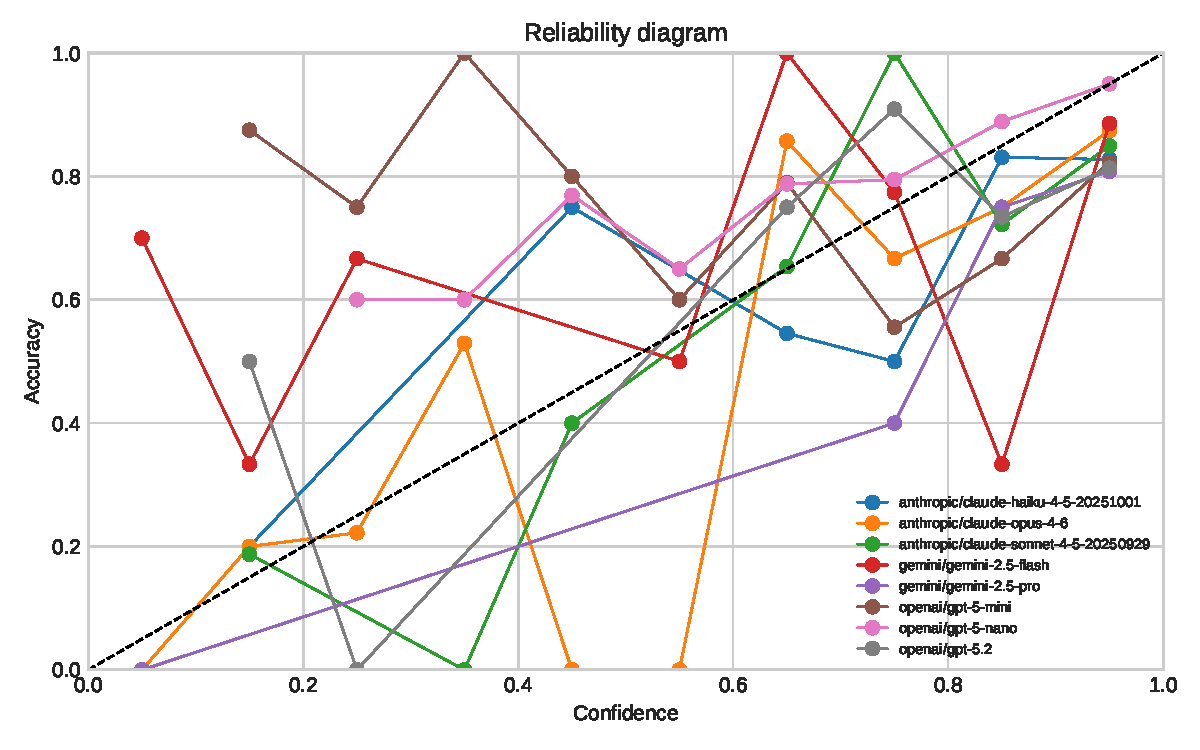
\includegraphics[width=0.9\linewidth]{figures/fig2_reliability_diagram_overlay.pdf}}{}
\caption{Reliability diagram (qualitative) under the operational chrF-based label.}
\label{fig:reliability}
\end{figure}

\section{Discussion and limitations}
The main finding is comparative and operational: under one shared protocol, self-reported confidence behaves as a provider-dependent score, so fixed thresholds induce different routing/abstention points. This does not imply semantic calibration.

Limitations remain explicit: (i) target is operational chrF/BLEU overlap, not semantic correctness; (ii) no completed human semantic-audit labels; (iii) no bundled non-baseline prompt-variant outputs; (iv) one language pair/dataset with 500 sentences; (v) parse-warning burden (443/4000) is an implementation-level confound.

Full prompts, mismatch examples, robustness exports, and artifact-level provenance are included in the accompanying repository.

\section{Conclusion}
Across 500 WMT17 sentences and 4,000 outputs from eight LLMs, confidence portability fails under a shared black-box MT protocol: similar mean chrF coexists with large cross-provider gaps in ECE and mismatch@0.9. The central claim is practical and scoped to this operational target.

Provider-specific isotonic calibration may mitigate alignment within providers, but it does not restore a shared probability scale across providers. Deployment should therefore use provider-specific threshold tuning/calibration or stronger external evaluator layers rather than assuming universal threshold portability.

\bibliographystyle{plainnat}
\bibliography{references,added_refs}
\end{document}
